\section{Evaluation}\label{sec:eval}
This section reports on our extensive evaluation of \SYS{}.
First, we present our evaluation settings.
Then, we describe the real-world dataset used in our macro-benchmark experiments.
We then dig into a set of micro-benchmarks that evaluate the overhead of running the \textsc{LuaVM} inside the SGX enclaves.
Finally, we deploy a full \SYS{} pipeline, scaling the number of workers per stage, to study the limits of the system in terms of throughput and scalability.


\subsection{Evaluation Settings.}
We have experimented on machines using a processor Intel$^{\tiny{\textregistered}}$~Core\texttrademark~i7-6700~\cite{intel:i7_6700} and $8\,GB$ RAM.
We use a cluster of 2 machines based on \textsc{Ubuntu} 14.04.1 LTS (kernel 4.2.0-42-generic).
The choice of the Linux distribution is driven by compatibility reasons with the latest Intel SGX SDK. 
The machines run Docker (v.1.13.0) and each node joins a Docker Swarm~\cite{docker:swarm_2016} (v1.2.5) using the Consul~\cite{consul} (v0.5.2) discovery service.
The Swarm manager and the discovery service are deployed on a distinct machine.
Containers leverage the Docker overlay network to communicate to each other.
Machines are interconnected using a switched $1\,Gbps$ network.

%\vs{add SGX things}
%\ah{in SGX things, explain the choice of Ubuntu 14.04.1}
%\ah{should we reference public repositories and specific version (commit hashes) of used stuff (driver, platform) for SGX?}


\subsection{Input Dataset.}
In our experiments, we process a real dataset released by the \emph{American Bureau of Transportation Statistic}~\cite{rita:bts}.
The dataset reports on the flight departures and arrivals of $20$ air carriers~\cite{statistical_computing:data}.
We implement a benchmark application atop of \SYS{} to compute average delays and the total of delayed flights for each air carrier.
We design and implement the full processing pipeline, that (i) parses the input datasets (in a comma-separated-value format) to data structure (\textsf{map}), (ii) filters data by relevancy (\emph{i.e.}, if the data concerns a delayed flight), and (iii) finally reduces it to compute the wanted informations.\footnote{This experiment is inspired by Kevin Webber's blog entry \emph{Diving into Akka Streams}: \url{https://blog.redelastic.com/diving-into-akka-streams-2770b3aeabb0}.}
We use the $4$ last years of the available dataset (from 2005 to 2008), for a total of $28$ millions of entries to process and $2.73\,GB$ of data.
%\vs{Update with the details of other datasets if any}
%\ah{wouldn't it be more logical to puts Dataset section after Micro-Benchmark one?}

\subsection{Micro-Benchmark: \textsc{Lua} in SGX.}
We begin our evaluation by a set of micro-benchmarks to evaluate performance of the integration of the \textsc{LuaVM} inside the SGX enclaves.
First, we estimate the cost of execution for functions inside the enclave.
This test averages the execution time of 1 million function calls, without any data transfer.
%  enclaved function calls we averaged the time it took to do one milion calls with no data transfers.
We compare against the same result on a vanilla \textsc{Lua} virtual machine.
While non-enclaved function calls took $23.6\,ns$, the performances inside enclave drop down to on average $2.35\,\mu{}s$---\textit{i.e}., approximately two orders of magnitude worse.
We then assess the cost of copying data from the unshielded, vanilla \textsc{Lua}~VM execution to the enclave and we compare it with the time required to compute the same on the native system.
We initialize a buffer of $100\,MB$ with random data and copy its content inside the enclave. 
The data is split into chunks of increasing sizes.
Our test executes one function call to transfer each chunk, until all data is transfered.
Each point in the plot corresponds to the average of $20$ runs. 
Correctness of the copies was verified by \textsf{SHA256} digest comparison between reproduced memory areas.
Figure~\ref{fig:sgxmemcpy} shows the results for 4 different variants, comparing the Native and the SGX version to only copy the data inside the enclave (\emph{in}) or to copy it inside and copying it back (\emph{in\/out}).
When using smaller chunks, the function call overhead plays an important role in the total execution time.
Moreover, we notice that the call overhead steadily drops until the chunk size reaches the size of $64\,KB$ (vertical line).
We can also notice that copying data back to non-SGX execution impose an overhead of at most $20\,\%$ when compared to the one-way copy.
These initial results can be used as guidelines to drive the configuration of the streaming pipeline, in particular with respect to the size of the chunks. %confirm that for the envisioned target scenarios of \SYS, our chosen runtime performs reasonably well compared to a native yet non-trusted framework.

\begin{figure}[t!]
  \centering
  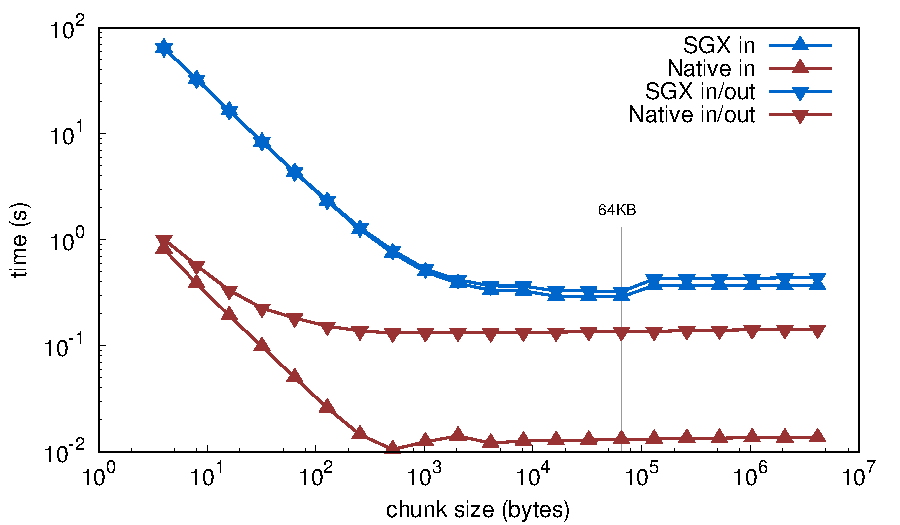
\includegraphics[width=\linewidth]{plots/memcpy/memcpy}
  \caption{Execution time to copy $100\,MB$ of memory inside an SGX enclave (\emph{in}) or to copy it back outside {\emph{in/out}.} }
  \label{fig:sgxmemcpy}
\end{figure}

Once the data and the code are copied inside the enclave, the Lua VM must indeed executes the code before returning the control. 
Hence, we evaluate here the raw performances of the enclaved SGX Lua VM.
We select $6$ available benchmarks from a standard suite of tests~\cite{bolz2015}.
We based this choice on their library dependencies (by selecting the most standalone ones) and the number of input/output instructions they execute (selecting those with the fewest I/O).
Each benchmark runs $20$ times with the same pair of parameters of the original paper, shown in the even and odd lines of Table~\ref{tab:luabmarks}.
%Again, we compare the results of the vanilla VM against the our SGX Lua interpreter.
Figure~\ref{fig:luabenchs} depicts the total time (average and standard deviation) required to complete the execution of the 6 benchmarks.
We use a bar chart plot, where we compare the results of the \emph{Native} and \emph{SGX} modes. 
For each of the $6$ benchmarks, we present two bars next to each other (one per executing mode) to indicate the different configuration parameters used.
Finally, for the sake of readability, we use a different y-axis scale for the \textsf{binarytrees} case (from $0$ to $400$\,seconds), on the right-side of the figure.

\newcommand{\higparamcolor}{\rowcolor[rgb]{0.79,0.91,0.90}\cellcolor{white}}
\newcommand{\lowparamcolor}{\rowcolor[rgb]{0.94,0.88,0.76}\cellcolor{white}}
\begin{table}[t!]
    \centering
    \begin{tabular}{r|c|c|c}
   % \hline
                       &configuration &memory      &ratio \\
                       &parameter     &peak        &SGX/Native \\
\hline
\lowparamcolor
\textsf{dhrystone}     &50\,K      &275\,KB       & 1.14 \\
\higparamcolor
                       &5\,M       &275\,KB       & 1.04 \\
\hline
\lowparamcolor
\textsf{fannkuchredux} &10         &28\,KB        & 0.99 \\
\higparamcolor
                       &11         &28\,KB        & 1.04 \\
\hline
\lowparamcolor
\textsf{nbody}         &2.5\,M     &38\,KB        & 0.99 \\
\higparamcolor
                       &25\,M      &38\,KB        & 1.00 \\
\hline
\lowparamcolor
\textsf{richards}      &10         &106\,KB       & 1.02 \\
\higparamcolor
                       &100        &191\,KB       & 0.97 \\
\hline
\lowparamcolor
\textsf{spectralnorm}  &500        &52\,KB        & 1.00 \\
\higparamcolor
                       &5\,K       &404\,KB       & 0.99 \\
\hline
\lowparamcolor
\textsf{binarytrees}   &14         &25\,MB        & 1.18 \\
\higparamcolor
                       &19         &664\,MB       & 4.76 \\
  %  \hline
    \end{tabular}
    \caption{Parameters and memory usage for \textsc{Lua} benchmarks.}
  \label{tab:luabmarks}
\end{table}

\begin{figure}[t!]
  \centering
  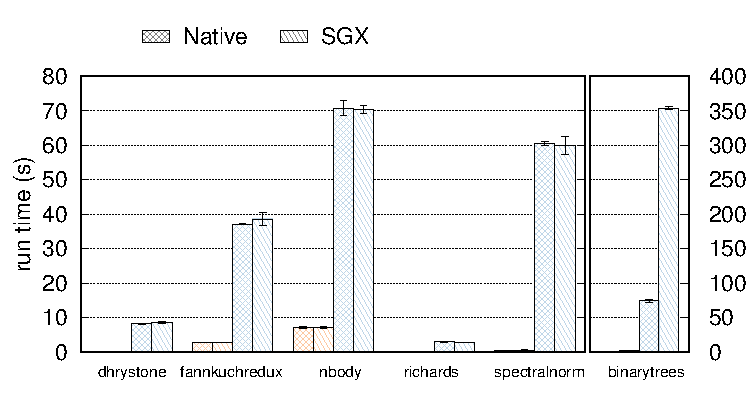
\includegraphics[width=\linewidth]{plots/microbenchmark_luasgx/microbenchmark_luasgx}
  \caption{Enclave versus native running times for \textsc{Lua} benchmarks}
  \label{fig:luabenchs}
\end{figure}

We note that, in the current version of SGX, it is required to pre-allocate all the memory area to be used by the enclave. 
The most memory-eager test (\textsf{binarytrees}) used more than $600\,MB$ of memory, hence using the wall clock time comparison would not be fair for for smaller tests.
In such cases, almost the whole execution time is dedicated to memory allocation.
Because of that, we subtracted the allocation time from the measurements of enclave executions, based on the average for the $20$ runs.
Fluctuations on this measurement produced slight variations in the execution times, sometimes producing the unexpected result of having SGX executions faster than native ones (by at most $3\,\%$).
Table~\ref{tab:luabmarks} lists the parameters along with the maximum amount of memory used and the ratio between runtimes of SGX and Native executions.
When the memory usage is low, the ratio between the Native and SGX versions is small---\emph{e.g.}, less than $15\,\%$ in our experiments. 
However, when the amount of memory usage increases, performance drops to almost 5$\times$ worse, as reflected in the case of the \emph{binarytrees} experiment.

\subsection{Benchmark: Upload Throughput}
The previous set of experiments allowed us to verify that our design, implementation, and the integration of the \textsc{LuaVM} into the SGX enclaves is sound.
Next, we deploy a \SYS{} pipeline which includes mappers, filters and reducers.
To measure the achievable throughput of our system, as well the network overhead of our architecture, 
we deploy the \SYS{} pipeline in 3 different configurations.
The first configuration allows the streaming framework to blindly bypass the SGX enclaves.
Further, it does not encrypt the input dataset before injecting it into the pipeline.
This mode operates as the baseline, yet completely \emph{unsafe}, processing pipeline.
The second mode encrypts the dataset but let the encrypted packets skip the SGX enclaves.
This configuration requires the deployers to trust the infrastructure operator.
Finally, we deploy third, fully secure pipeline, where the input dataset is encrypted and the data processing is operated inside the enclaves.
The results of these deployments are presented in Figure~\ref{fig:throughput}.
For each of the mentioned configurations, we also vary the number of workers per stage, from one (Figure~\ref{fig:throughput}-a,d,g), two (Figure~\ref{fig:throughput}-b,e,h), or four (the remaining ones.)
\vs{stopped here}
This benchmark shows the upload throughput observed across the whole cluster while streaming the dataset as fast as possible from the source nodes into the processing pipeline.
We gather bandwidth measurements by exploiting Docker's internal monitoring and statistical module.
%Throughput accross containers wrapping each node of the processing pipeline are measured from Docker stats.
The statistics are gathered at runtime while the experiment is executing.
%During the experiment, we retrieve all the data stats for each container.
%In particular, \texttt{txbytes} stats are extracted to measure containers output throughput.
We report on our results in Figure~\ref{fig:throughput}.
In this scenario, 4 nodes concurrently inject the input dataset into the processing pipeline, each one using a subset of the full dataset.
However, only one worker process is used for each step of the processing pipeline.
We use a representation based on stacked percentiles.
The white bar at the bottom represents the minimum value, the pale grey on top the maximal value.
Intermediate shades of grey represent the 25th-, 50th–, median–, and 75th-percentiles.
For instance, the median throughput at 200\,seconds into the experiment almost hits $2,500\,kB/s$, meaning that $50\,\%$ of the nodes in that moment are outputting data at $2,500\,kB/s$ or less.
%These datas are computed to be plotted together by percentile, as shown on figure \ref{fig:throughput}.\ah{maybe it could be relevant to put three plots, corresponding to experiments 4-datas-1-worker, 4-datas-2-workers and 4-datas-4-workers}
With the current implementation, we observe a peak of $10\,MB/s$ upload throughput into the processing stages.%\vs{for the future, it'd be interesting to know which stage is the fastest one}
%\ah{I gonna measure throuput between two containers run on a swarm cluster, using iperf, for comparison purpose}


\vs{We should then extend this section to present how the TPUT is affected by having few/all streams going through the enclaves. This would be an interesting/useful plot as it provides useful insights.}


\subsection{Benchmark: Workers Scalability}
We conclude this evaluation by presenting scalability results of the \SYS{} framework.
In particular, we scale up each stage of the processing pipeline, up to 4\,workers per stage.
For each of the configurations, the experiment is repeated 20\,times.
We show average and standard deviation of the overall completion time to process the full dataset.
Figure~\ref{fig:scalability} depicts these results.
%Scalability of \SYS is evaluated by processing these datas 20 times on 3 different pipeline topology: using 1, 2 or 4 workers for each step of the pipeline.
We observe that by doubling the number of workers from the initial configuration achieves a 2$\times$ speed-up of the overall processing time, that is from 20\,minutes to less than 10\,minutes.
Conversely, we do not observe similar improvements when using 4\,workers.
%Results are represented on figure \ref{fig:scalability}, and show clearly better performances between the experiment using only one worker by task, and the one using 2 workers.
%In an other hand, using 4 workers instead of 2 does not show any performance improvement.

\begin{figure}[t!]
  \centering
  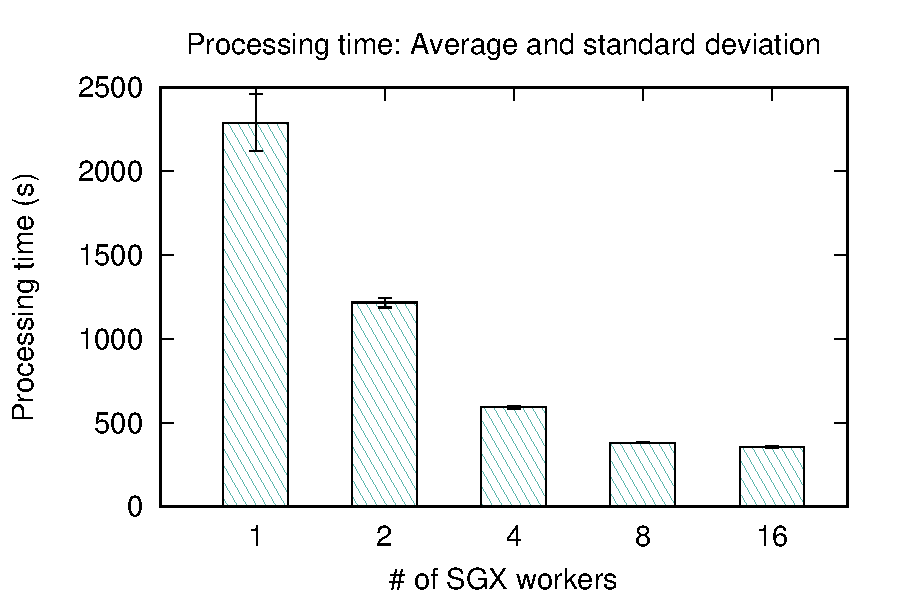
\includegraphics[width=\linewidth]{plots/secure_streams/scalability/sgxmapper_scalability}
  \caption{Scalability: processing time, average and standard deviation. The experiment is repeated 5\,times, with a variation on the number of mappers SGX, other workers - 1 filter worker and 1 reduce worker - do not use SGX.}
  \label{fig:scalability}
\end{figure}

We believe this behavior can be explained by existing bottlenecks in the pipelining infrastructure, the lack of optimization in the application logic as well as tuning options of the \zmq{} queues.
These hypotheses are confirmed by observing the throughput of the system when we increase the processing workers to 2 and 4 in Figure~\ref{fig:throughput2} and Figure~\ref{fig:throughput4}, respectively.
We observe the following facts.
First, the system is far from saturating the network's available bandwidth, hitting a peak of $10\,MB/s$.
Second, a small percentage of nodes consumes much more bandwidth than the other components.
We intend to further investigate these effects as part of our future work, as we are going to elaborate in the following section.

\begin{figure*}[!t]
\centering
\begin{tabular}{cccc}
\subfloat[Throughput without encoding]{
  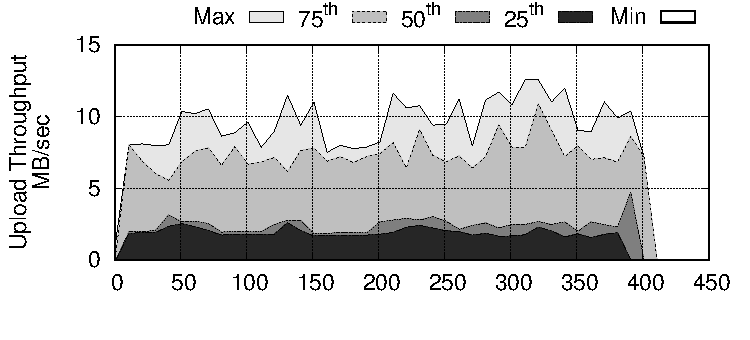
\includegraphics[width=.31\linewidth]{plots/secure_streams/throughput/tput_tx_percentiles_1-workers}
} &
\subfloat[Throughput without SGX]{
  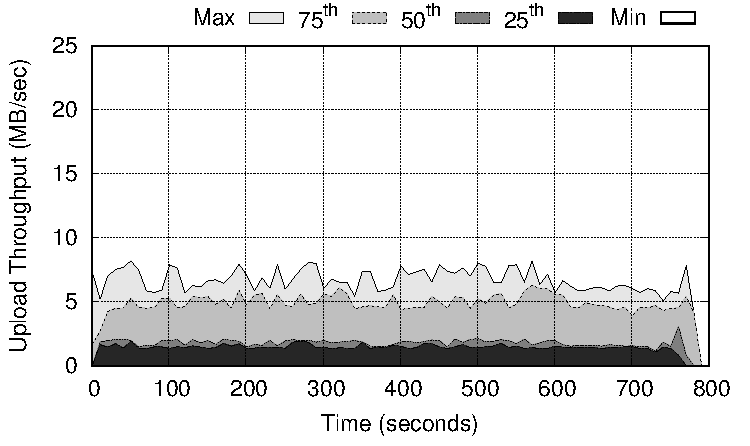
\includegraphics[width=.31\linewidth]{plots/secure_streams/throughput/tput_tx_percentiles_1-workers-encrypted-nosgx}
} &
\subfloat[Throughput with SGX]{
  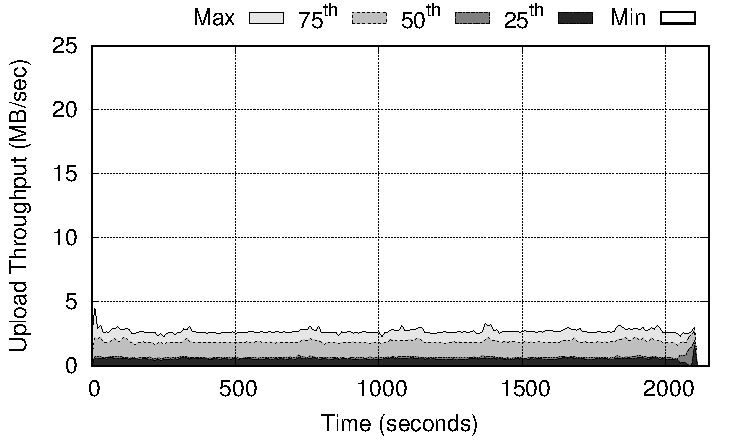
\includegraphics[width=.31\linewidth]{plots/secure_streams/throughput/tput_tx_percentiles_1-workers-encrypted-fullsgx}
}\cr
\subfloat[Throughput without encoding]{
  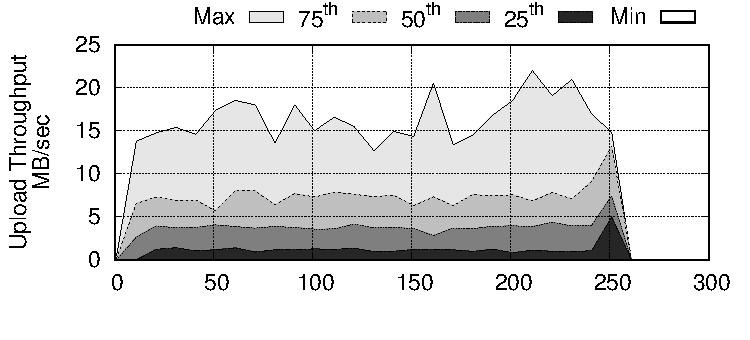
\includegraphics[width=.31\linewidth]{plots/secure_streams/throughput/tput_tx_percentiles_2-workers}
} &
\subfloat[Throughput without SGX]{
  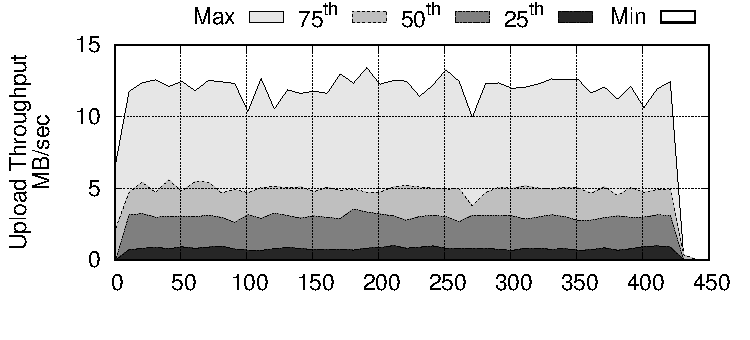
\includegraphics[width=.31\linewidth]{plots/secure_streams/throughput/tput_tx_percentiles_2-workers-encrypted-nosgx}
} &
\subfloat[Throughput with SGX]{
  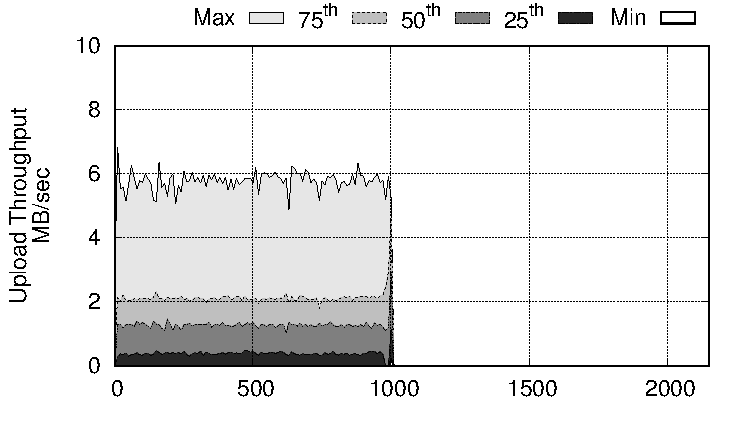
\includegraphics[width=.31\linewidth]{plots/secure_streams/throughput/tput_tx_percentiles_2-workers-encrypted-fullsgx}
}\cr
\subfloat[Throughput without encoding]{
  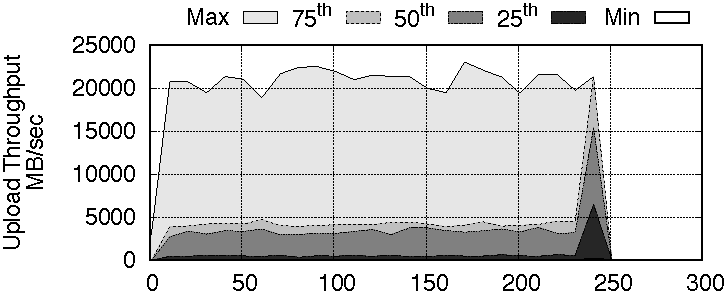
\includegraphics[width=.31\linewidth]{plots/secure_streams/throughput/tput_tx_percentiles_4-workers}
} &
\subfloat[Throughput without SGX]{
  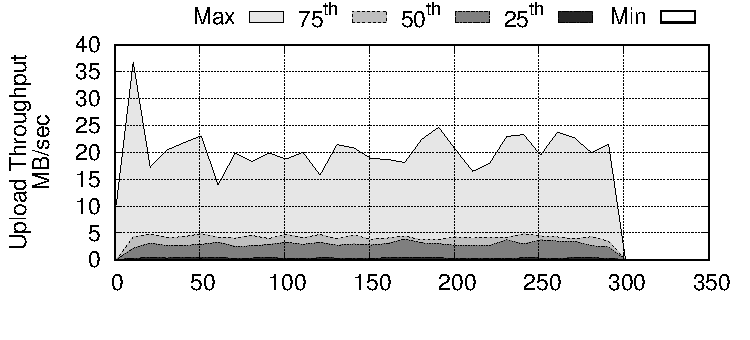
\includegraphics[width=.31\linewidth]{plots/secure_streams/throughput/tput_tx_percentiles_4-workers-encrypted-nosgx}
} &
\subfloat[Throughput with SGX]{
  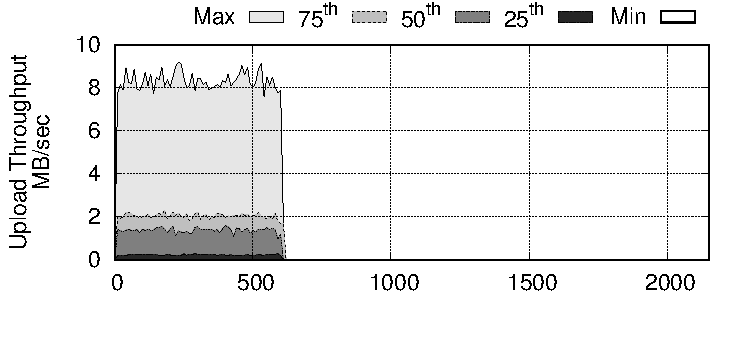
\includegraphics[width=.31\linewidth]{plots/secure_streams/throughput/tput_tx_percentiles_4-workers-encrypted-fullsgx}
}
\end{tabular}
\caption{Throughput comparison between normal processing and SGX processing}
\end{figure*}

